
\documentclass[10pt]{beamer}
%\documentclass[10pt,handout]{beamer}
%\documentclass{beamer}

\usepackage{amsmath}
\usepackage{amssymb}
\usepackage{latexsym}
\usepackage{epsfig}
\usepackage{graphics}
\usepackage{graphicx}
\usepackage[normalem]{ulem}
\usepackage{amsmath}

\graphicspath{ {images/} }

\mode<presentation>
{
\usetheme{Warsaw}
%\setbeamercovered{dynamic}
\setbeamercolor{palette primary}{bg=blue}
\setbeamercolor{block title}{bg=blue}
\setbeamercolor{lowercol}{bg=green}
}
\setbeamertemplate{navigation symbols}{}

\pgfdeclareimage[height=.9cm]{AULogo2}{SampTA2011Figs/AULogo2} \logo{\pgfuseimage{AULogo2}}

%==========================(Casey's LaTeX Shortcuts)================================
%===================================================================================

% SYMBOLS %
% ---------------------- Blackboard Bold --------------------------------
\def\R{\mathbb{R}}                     % real numbers R
\def\C{\mathbb{C}}                     % complex numbers C
\def\N{\mathbb{N}}                     % natural numbers
\def\Z{\mathbb{Z}}                     % integers
\def\Q{\mathbb{Q}}                     % rational numbers
\def\P{\mathbb{P}}                     % primes
\def\W{\mathbb{W}}                     % windowing functions
\def\B{\mathbb{B}}                     % partition of unity functions
\def\A{\mathbb{A}}                     % almost orthogonal windowing functions
\def\T{\mathbb{T}}                     % unit circle (\R mod 2 \pi)
\def\F{\mathbb{F}}                     % Functions
\def\I{\mathbb{I}}                     % Intervals
\def\D{\mathbb{D}}                     % The unit disk
\def\Rn{{\R}^{n}}                      % n-dimensional R space
\def\Cn{{\C}^{n}}                      % n-dimensional C space
\def\Rhat{{\widehat{\R}}}              % reals (dual)
\def\Rnhat{{\widehat{\Rn}}}            % n-dim reals (dual)
\def\PW{\mathbb{PW}}                   % Paley-Wiener Space

% WORD FUNCTIONS %
\def\sinc{\mathop{\textstyle{\rm sinc}}}
\def\domain{\mathop{\textstyle{\rm Domain}}\nolimits}
\def\essinf{\mathop{\textstyle{\rm ess \, inf}}}
\def\esssup{\mathop{\textstyle{\rm ess \, sup}}}
\def\range{\mathop{\textstyle{\rm Range}}\nolimits}
\def\Span{\mathop{\textstyle{\rm span}}\nolimits}
\def\supp{\mathop{\textstyle{\rm supp}}\nolimits}
\def\CHI{\hbox{\raise .5ex \hbox{$\chi$}}}
\def\Tri{\mbox{Tri}}
\def\Trap{\mbox{Trap}}
\def\Cap{\mbox{Cap}}
\def\loc{{\textstyle{\rm loc}}}
\def\qed{ \hspace*{\fill} \Q \mathbb{E} \D}
% \def\qed{ \hspace*{\fill} \Box}

% UNARY, BINARY OPERATORS %
\def\norm#1{\|  #1 \|}
\def\abs#1{| #1 |}
\def\bigabs#1{\biggl| #1 \biggr|}
\def\set#1{\{ #1 \}}
\def\bigset#1{\biggl\{ #1 \biggr\}}
\def\ceiling#1{\lceil #1 \rceil}
\def\floor#1{\lfloor #1 \rfloor}
\def\ip#1#2{\langle #1 , #2 \rangle}
\def\bigip#1#2{\bigl\langle #1, \, #2 \bigr\rangle}
\def\Bigip#1#2{\Bigl\langle #1, \; #2 \Bigr\rangle}
\def\biggip#1#2{\biggl\langle #1, \; #2 \biggr\rangle}
\def\ipsize#1#2{\left\langle #1 , #2 \right\rangle}
\def\Int#1{\lfloor #1 \rfloor}
\def\biggInt#1{\biggl\lfloor #1 \biggr\rfloor}
\def\Intsize#1{\left\lfloor #1 \right\rfloor}
\def\paren#1{( #1 )}
\def\bigparen#1{\left( #1 \right)}
\def\Bigparen#1{\Bigl( #1 \Bigr)}
\def\biggparen#1{\biggl( #1 \biggr)}
\def\Biggparen#1{\Biggl( #1 \Biggr)}
\def\sqparen#1{[ #1 ]}
\def\bigsqparen#1{\biggl[ #1 \biggr]}

\newcommand{\hl}[1]{{\bf #1}}
\newcommand{\refp}[1]{(\ref{#1})}

\newcommand{\stkout}[1]{\ifmmode\text{\sout{\ensuremath{#1}}}\else\sout{#1}\fi}

\def\comment#1{}

%==========================(End of my LaTeX Commands)===============================
%

%\begin{document}

\title{
  {\bf{\textsf{
        Let $\epsilon > 0$ Be Given
}}}}

\author[Erik Taubeneck]{Erik Taubeneck}

\institute[GameChanger]
{
{GameChanger}
}

\date{November 16th, 2016}

\begin{document}

% Creates title page of slide show using above information
\begin{frame}
  \titlepage
\end{frame}

%\section[Outline]{}

% Creates table of contents slide incorporating
% all \section and \subsection commands

\begin{frame}
  \frametitle{The Beginning of the Story}

\center{
  
\includegraphics[scale=0.2]{first_day.png}
}

\end{frame}

\begin{frame}
  \frametitle{The Beginning of the Story}

\center{
  \includegraphics[scale=0.5]{geb.jpg}
} \pause

\center{ Propositional Calculus }

\end{frame}

\begin{frame}
  \frametitle{The Beginning of the Story}

\center{
  \includegraphics[scale=0.5]{geb.jpg}
}

\center{ \stkout{Propositional} Calculus }

\end{frame}


\begin{frame}
  \frametitle{The \textit{Real} Beginning of the Story}

  \begin{minipage}{4in}
    \centering
    \raisebox{-0.5\height}{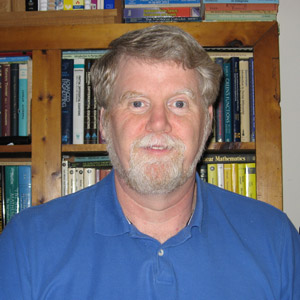
\includegraphics[height=1.75in]{doc_kc.jpg}}
    \hspace*{.2in}
    \raisebox{-0.5\height}{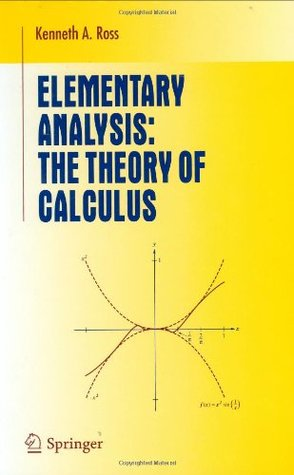
\includegraphics[height=1.75in]{ross_elementary_analysis.jpg}}
  \end{minipage}
\end{frame}


\begin{frame}
  \frametitle{Elementary Analysis}

  Outline:
  \begin{itemize}
  \item $\N$: The \textit{natural numbers} (i.e. counting numbers)
  \item $\Z$: The \textit{integers} (i.e. $\N$ $\cup$ 0 $\cup$ negative $\N$)
  \item $\Q$: The \textit{rational numbers} (i.e. fractions)
  \item $\R$: The \textit{real numbers} (i.e. $\Q$ $\cup$ the crazy numbers like $e$ and $\pi$)
  \item Sequence: a sequence of numbers, (e.g. $\{1, 1, 2, 3, 5, 8, ...\}$)
  \item $\infty$ (infinity)
  \item Hyper-dimensional balls in crazy high dimensions
  \end{itemize}
\end{frame}

\begin{frame}
  \frametitle{Math - The Universal Language?}
  \center{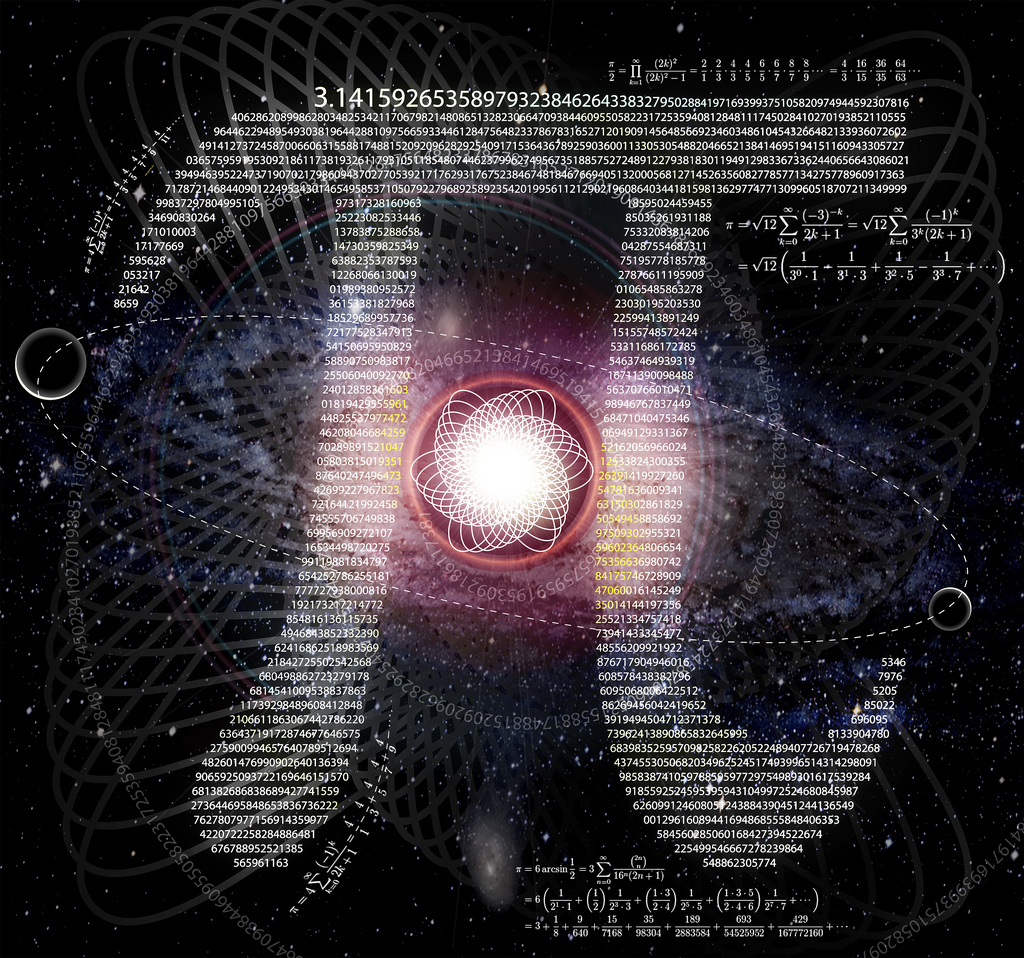
\includegraphics[scale=0.75]{universal_language.jpg}}
\end{frame}

\begin{frame}
  \frametitle{Nope!}
  \center{
\includegraphics[scale=0.25]{universal_language_nope.png}}
\end{frame}

\begin{frame}
  \frametitle{Math is rooted in Definitions and Axioms}
  \center{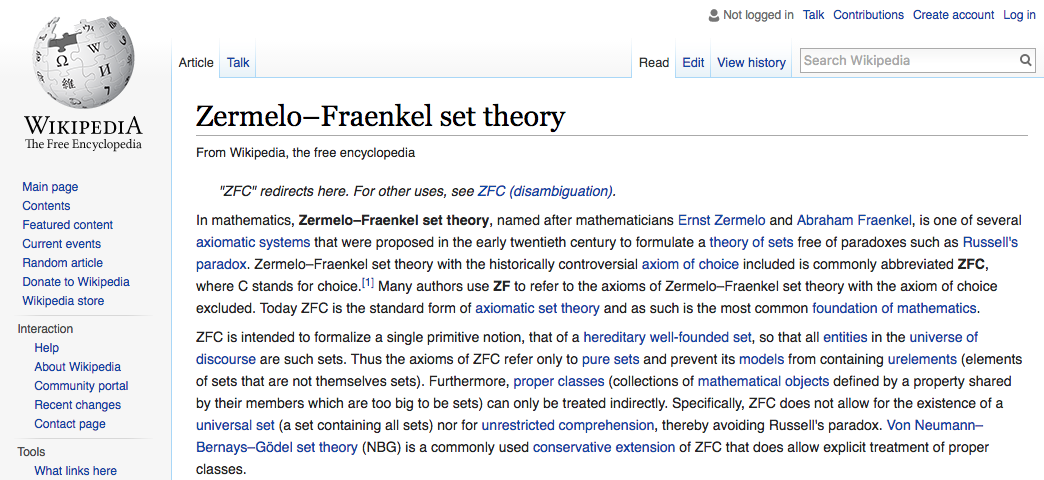
\includegraphics[scale=0.3]{zfc.png}}
\end{frame}

\begin{frame}
  \frametitle{Natural Numbers}

  \[ \N = {1, 2, 3, ...} \]

  \pause

  We define the \textit{natural numbers} $\N$ by the following axioms: \pause

  \begin{itemize}
  \item N1. $1 \in \N$ \pause
  \item N2. If $n \in \N$, then its successor $n + 1 \in \N$. \pause
  \item N3. 1 is not the successor of any element of $\N$. \pause
  \item N4. If $n$ and $m$ have the same successors, then $n = m$. \pause
  \item N5. A subset of $\N$ which contains 1, and which contains $n + 1$ whenever it contains n, must equal $\N$.
  \end{itemize}
\end{frame}

\begin{frame}
  \frametitle{Integers, Rationals, and Reals}

  \begin{itemize}
  \item $\Z = \N \cup \{0\} \cup \{ -n $ for all $n \in \N \}$ \pause
  \item $\Q = \{ \frac{p}{q} $ for all $p, q \in \Z$, $q \ne 0\}$. \pause
  \item $\R$ (talk to me afterwards...)
  \end{itemize}
\end{frame}

\begin{frame}
  \frametitle{Sequences}

  A \textit{sequence} is a function $s(n)$ (often denoted as $s_n$) who's domain is $\N$. \pause

  \textbf{Examples}:

  \begin{itemize}
  \item $\left ( 1, 2, 3, ... \right ): s_n = n$ \pause
  \item $\left ( 1, 1, 2, 3, 5, 8, ... \right ): s_1 = 1; s_2 = 1; s_n = s_{n-1}$ \pause
  \item $\left ( 1, \frac{1}{2}, \frac{1}{4}, \frac{1}{8}, ... \right ): s_n = \frac{1}{n^2}$ \pause
  \item $\left ( -1, 1, -1, 1, -1, ... \right ): s_n = -1^n$ \pause
  \item $\left ( 2, \left ( \frac{3}{2} \right )^2, \left ( \frac{4}{3} \right )^3, \left ( \frac{5}{4} \right )^4, ... \right ): s_n = \left ( 1 + \frac{1}{n} \right )^n$ \pause
  \item $\left ( \frac{1}{2}, -\frac{1}{2}, -1, -\frac{1}{2}, \frac{1}{2}, 1, \frac{1}{2},
    -\frac{1}{2}, -1, -\frac{1}{2}, \frac{1}{2}, 1, ... \right ): s_n = \cos \left ( \frac{n \pi}{3} \right )$
  \end{itemize}

\end{frame}

\begin{frame}
  \frametitle{Infinity}

  When working with a \textit{sequence} $s$, we often want to find out the limit of $s_n$ as $n \to \infty$. \pause
  \vspace{5mm}

  Unfortunately, $\infty$ isn't a \textit{number}, but instead a process. Thus we cannot simply calculate $s_{\infty}$. \pause
  \vspace{5mm}

  A \textit{sequence} can do one of three things as $n \to \infty$:

  \begin{itemize}
  \item Converge to $m \in \R$
  \item Diverge to $\infty$ or $-\infty$
  \item Not Converge or Diverge
  \end{itemize}

  Each of these has their own definition.
  \vspace{5mm}

\end{frame}

\begin{frame}
  \frametitle{Convergent Sequences}

  A \textit{sequence} is said to \textit{converge} to $s \in \R$ if for any $\epsilon > 0$ there exists an $N \in \N$ such that $\vert s_n - s \vert > \epsilon$ for all $n > N$ ($n \in \N$). \pause
  \vspace{5mm}

  \textbf{Example:} Prove that $s_n = \frac{1}{n}$ converges to $s = 0$. \pause
  \vspace{5mm}

  \textbf{Proof:} Let $\epsilon > 0$ be given. \pause Let $N = \left \lceil \frac{1}{\epsilon} \right \rceil$. Then, for all $n > N$, \pause

  \[ N \ge \frac{1}{\epsilon} \text{ and } \frac{1}{n} < \frac{1}{N}. \] \pause

  Thus,

  \[ \left \vert s_n - s \right \vert = \left \vert s_n - 0 \right \vert =  \left \vert s_n \right \vert =
  \left \vert \frac{1}{n} \right \vert < \frac{1}{N} \le \epsilon \] \pause

  and therefore

  \[ \left \vert s_n - s \right \vert < \epsilon. \] \pause

  $\qed$

\end{frame}


\begin{frame}
  \frametitle{Divergent Sequences}

  A \textit{sequence} is said to \textit{diverge} if for any $M > 0$ there exists an $N \in \N$ such that $s_n > M$ for all $n > N$ ($n \in \N$). \pause
  \vspace{5mm}

  \textbf{Example:} Prove that $s_n = n$ diverges. \pause
  \vspace{5mm}

  \textbf{Proof:} Let $M>0$ be given. \pause Let $N = \lceil M \rceil$. \pause Then, for all $n > N$,

  \[ M \le N < n = s_n \] \pause

  and therefore

  \[ M < s_n. \] \pause

  $\qed$

\end{frame}

\begin{frame}
  \frametitle{Divergent Sequences}

  A \textit{sequence} is said to \textit{diverge} if for any $M > 0$ there exists an $N \in \N$ such that $s_n > M$ for all $n > N$ ($n \in \N$).
  \vspace{5mm}

  \textbf{Example 2:} Prove that $s_n = \frac{n}{2}$ diverges. \pause
  \vspace{5mm}

  \textbf{Proof:} Let $M > 0$ be given. \pause Let $N = \lceil 2M \rceil $. Then, for all $n > N$, \pause

  \[ \frac{n}{2} > \frac{N}{2} \text{ and } \frac{N}{2} \le M. \] \pause

  Thus,

  \[ M \le \frac{N}{2} < \frac{n}{2} = s_n \] \pause

  and therefore

  \[ M < s_n. \] \pause

  $\qed$

\end{frame}




\begin{frame}
  \frametitle{Infinity}

  \[ \lim_{n \to \infty} s_n = 0 \]

  \[ \lim_{n \to \infty} s_n = \infty \]

\end{frame}

\begin{frame}
  \frametitle{Infinity}


  \[ \stkout{ \lim_{n \to \infty} s_n = 0 } \]

  A \textit{sequence} is said to \textit{converge} to $s \in \R$ if for any $\epsilon > 0$ there exists an $N \in \N$ such that $\vert s_n - s \vert > \epsilon$ for all $n > N$ ($n \in \N$).

  \[ \stkout{ \lim_{n \to \infty} s_n = \infty } \]

  A \textit{sequence} is said to \textit{diverge} if for any $M > 0$ there exists an $N \in \N$ such that $s_n > M$ for all $n > N$ ($n \in \N$).


\end{frame}

\begin{frame}
  \frametitle{A Circle}

\setlength{\unitlength}{1mm}
\begin{picture}(10, 20)

\put(20,10){\circle{10}}
\put(50,10){\circle{5}}
\put(80,10){\circle{10}}
\put(80,10){\circle{5}}

\end{picture} \pause

Let $c_1$ be a circle with radius $=1$ and $c_{0.5}$ be a circle with radius $=0.5$. \pause
\vspace{5mm}

Then let $d$ be the "donut" left over when we remove $c_{0.5}$ from $c_1$. \pause
\vspace{5mm}

Now, let $A(x) = \pi r^2$ (the area function) and note that

\begin{tabular}{ l c r }
$A(c_1) = \pi$ & $A(c_{0.5}) = 0.25*\pi$ & A(d) = $A(c_1) - A(c_{0.5}) = 0.75\pi$ \\
\end{tabular}


\end{frame}


\begin{frame}
  \frametitle{A Circle}
  Now, note the proportion of area contained within the ``donut'' $d$

  \[ \frac{A(d)}{A(c_1)} =  \frac{A(c_1) - A(c_{0.5})}{A(c_1)} = \frac{0.75 \pi}{\pi} = 0.75 \]

\end{frame}


\begin{frame}
  \frametitle{A Sphere}

  \setlength{\unitlength}{1mm}
  \begin{picture}(20, 10)

    \put(20,10){\circle{10}}
    \put(50,10){\circle{5}}
    \put(80,10){\circle{10}}
    \put(80,10){\circle{5}}

  \end{picture} \pause

  Now, let $c_1^3$ be a sphere with radius $=1$ and

  $c_{0.5}^3$ be a sphere with radius $=0$. \pause
  \vspace{5mm}

  Then let $d^3$ be the "donut" left over when we remove $c_{0.5}$ from $c_1$. \pause
  \vspace{5mm}

  Now, let $V_3(x) = \frac{4}{3} \pi r^3$ (the volume function) and note that

  \begin{tabular}{ l c r }
    $V_3(c_1^3) = \frac{4}{3} \pi$ & $V_3(c_{0.5}^3) = \frac{4}{3} \frac{1}{2^3}*\pi = \frac{1}{6} \pi $ & $V_3(d^3) = V_3(c_1^3) - V_3(c_{0.5}^3) = \frac{7}{6} \pi$ \\
  \end{tabular}

\end{frame}

\begin{frame}
  \frametitle{A Sphere}

  Again, note the proportion of volume contained within the ``donut'' $d^3$

  \[ \frac{V_3(d^3)}{V_3(c_1^3)} =  \frac{V_3(c_1^3) - V_3(c_{0.5}^3)}{V_3(c_1^3)} = \frac{\frac{7}{6} \pi}{\frac{4}{3} \pi} = \frac{7}{8} \]


\end{frame}

\begin{frame}
  \frametitle{We Can Go Higher!}

  %% \setlength{\unitlength}{1mm}
  %% \begin{picture}(20, 10)

  %%   \put(20,10){\circle{10}}
  %%   \put(50,10){\circle{8}}
  %%   \put(80,10){\circle{10}}
  %%   \put(80,10){\circle{8}}

  %% \end{picture} \pause

  \setlength{\unitlength}{1mm}
  \begin{picture}(20, 10)

    \put(20,10){\circle{10}}
    \put(50,10){\circle{5}}
    \put(80,10){\circle{10}}
    \put(80,10){\circle{5}}

  \end{picture} \pause

  In general, the hyper-volume of a hyper-sphere in $n$ dimensions is

  \[ V_n(r) =  \frac{r^n \pi^{n/2}}{\Gamma (n/2 + 1)}. \] \pause

  Then, the proportion of volume contained within the hyper ``donut'' is

  \[ \frac{V_n(1) - V_n(0.5)}{V_n(1)} =  \frac{\frac{1^n \pi^{n/2}}{\Gamma (n/2 + 1)} -  \frac{(0.5)^n \pi^{n/2}}{\Gamma (n/2 + 1)}}{\frac{1^n \pi^{n/2}}{\Gamma (n/2 + 1)}} =
  \frac{\frac{(1-(0.5)^n) \pi^{n/2}}{\Gamma (n/2 + 1)}}{\frac{\pi^{n/2}}{\Gamma (n/2 + 1)}} = 1 - (0.5)^n \]

\end{frame}


  %% Now, for any $\epsilon > 0$, we can create a hyper donut that is arbitrarily close to the unit hyper sphere, but note that the hyper volume of the outer hyper donut is

  %% \[ V_n(1) - V_n(1-\epsilon) =  \frac{1^n \pi^{n/2}}{\Gamma (n/2 + 1)} -  \frac{(1-\epsilon)^n \pi^{n/2}}{\Gamma (n/2 + 1)} =
  %% \frac{(1-(1-\epsilon)^n) \pi^{n/2}}{\Gamma (n/2 + 1)} \]

\begin{frame}
  \frametitle{We Can Go Higher!}

  \setlength{\unitlength}{1mm}
  \begin{picture}(20, 10)

    \put(20,10){\circle{10}}
    \put(50,10){\circle{8}}
    \put(80,10){\circle{10}}
    \put(80,10){\circle{8}}

  \end{picture} \pause


  The proportion of volume contained within the hyper ``donut'' that is within $\delta > 0$, $\delta < 1$ of the surface is

  \[ \frac{V_n(1) - V_n(1-\delta)}{V_n(1)} =
  \frac{\frac{1^n \pi^{n/2}}{\Gamma (n/2 + 1)} -  \frac{(1-\delta)^n \pi^{n/2}}{\Gamma (n/2 + 1)}}{\frac{1^n \pi^{n/2}}{\Gamma (n/2 + 1)}} =
  \frac{\frac{(1-(1-\delta)^n) \pi^{n/2}}{\Gamma (n/2 + 1)}}{\frac{\pi^{n/2}}{\Gamma (n/2 + 1)}} = 1 - (1-\delta)^n \]

\end{frame}

\begin{frame}
  \frametitle{We Can Go Higher!}


  Let $s_n = 1 - (1-\delta)^n$. \pause

  \textbf{Claim:} $s_n$ converges to $s=1$ for all $\delta > 0, \delta < 1$. \pause
  \vspace{5mm}

  \textbf{Proof:} Let $\epsilon > 0$ be given \pause as well as $\delta > 0, \delta < 1$. \pause

  Let $N = \left \lceil \frac{\log (\epsilon)}{\log (1-\delta)} \right \rceil$. \pause Note that since $0 < \delta < 1$

  \[ \log (1 - \delta) < 1. \] \pause

  Then, for all $n > N$

\end{frame}

\begin{frame}
  \frametitle{We Can Go Higher!}

  \[ n > N \ge \frac{\log (\epsilon)}{\log (1-\delta)} \] \pause
  \vspace{-5mm}

  \[ n > \frac{\log (\epsilon)}{\log (1-\delta)} \] \pause
  \vspace{-5mm}

  \[ n \log (1-\delta) < \log (\epsilon) \] \pause
  \vspace{-5mm}

  \[ \log \left ( (1-\delta)^n \right ) < \log (\epsilon) \] \pause
  \vspace{-5mm}

  \[ (1 - \delta)^n < \epsilon \] \pause
  \vspace{-5mm}

  \[ 1 - (1 - (1-\delta)^n)) < \epsilon \] \pause
  \vspace{-5mm}

  \[ \left \vert 1 - (1 - (1-\delta)^n)) \right \vert < \epsilon \] \pause
  \vspace{-5mm}

  \[ \left \vert s - s_n \right \vert < \epsilon \]  \pause

  $\qed$

\end{frame}

\begin{frame}
  \frametitle{Woah!}

  \setlength{\unitlength}{1mm}
  \begin{picture}(20, 10)

    \put(20,10){\circle{10}}
    \put(50,10){\circle{8}}
    \put(80,10){\circle{10}}
    \put(80,10){\circle{8}}

  \end{picture}

  In crazy high enough dimensions, an arbitrarily high proportion of the outer hyper volume of any hyper sphere is concentrated arbitrarily close the boundary!

\end{frame}



\end{document}
